% Communication job: show two subsystem boundaries and their interface.
% Primary grammar: left-to-right grouped system architecture.
% Target geometry: single-column figure, natural width approximately 8.5 cm or less.
% Semantic status: schematic.
% Compile with: pdflatex system-architecture.tex
\documentclass[tikz,border=2mm,10pt]{standalone}

\usetikzlibrary{arrows.meta,positioning,fit,backgrounds}

\definecolor{figdark}{gray}{0.25}
\definecolor{figmid}{gray}{0.50}
\definecolor{figlight}{gray}{0.85}
\definecolor{figpale}{gray}{0.95}

\tikzset{
  block/.style={
    rectangle, draw=figdark, fill=figlight,
    minimum width=1.35cm, minimum height=0.75cm,
    align=center, inner sep=3pt
  },
  group/.style={
    rectangle, draw=figmid, dashed, fill=figpale,
    rounded corners=2pt, inner xsep=5pt,
    inner ysep=12pt
  },
  grouplabel/.style={font=\footnotesize, fill=figpale, inner sep=1pt},
  arrow/.style={->, >={Stealth[length=1.8mm]}, thick, draw=figdark},
  edgelabel/.style={font=\footnotesize, fill=white, inner sep=1pt}
}

\begin{document}
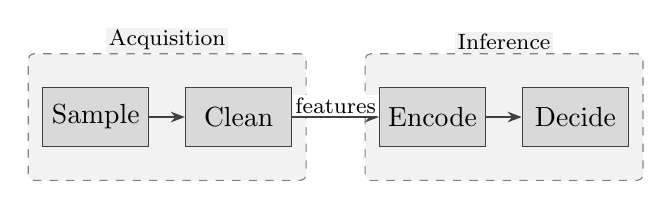
\begin{tikzpicture}[node distance=0.45cm]
  \node[block] (sample) {Sample};
  \node[block, right=of sample] (clean) {Clean};
  \node[block, right=1.10cm of clean] (encode) {Encode};
  \node[block, right=of encode] (decide) {Decide};

  \begin{scope}[on background layer]
    \node[group, fit=(sample)(clean),
      label={[grouplabel]above:Acquisition}] (acq) {};
    \node[group, fit=(encode)(decide),
      label={[grouplabel]above:Inference}] (inf) {};
  \end{scope}

  \draw[arrow] (sample) -- (clean);
  \draw[arrow] (clean) -- node[edgelabel, above] {features} (encode);
  \draw[arrow] (encode) -- (decide);
\end{tikzpicture}
\end{document}
